%File: functional-user.tex
%Date: Sat Oct 19 17:05:21 2013 +0800
%Author: Yikai Zhao <blahgeek@gmail.com>

\subsection{User Management}

An user's permitted behaviors on his/her account are included in but not
limited to the following:

\begin{itemize}
\itemsep1pt\parskip0pt\parsep0pt
\item
  Register an account
\item
  Login
\item
  Edit his/her personal profile
\item
  Change his/her password
\item
  Delete his/her account, along with all the relevant data
\end{itemize}

Moreover, since Uknow is supposed to connect to multiple diversed service providers,
users have to provide authorize us the use of their accounts on other web services.
OAuth\footnote{\url{http://oauth.net/}} is an open protocol to allow secure authorization.
By using OAuth, users can safely authorize Uknow to use their accounts.
The principles and proecss of OAuth authorization is illustrated in \figref{oauth}.

\begin{figure}[H]
  \centering
  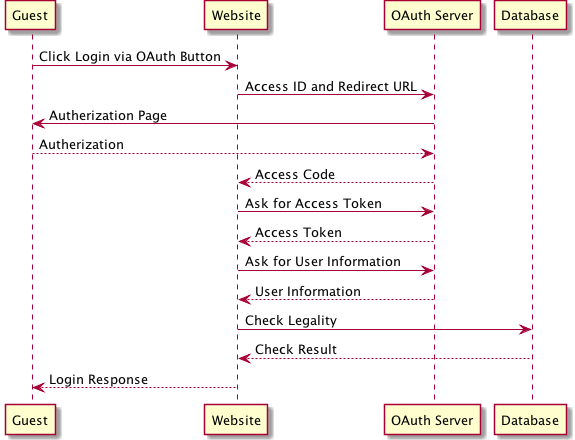
\includegraphics[width=0.8\textwidth]{img/oauth.png}
  \caption{OAuth process \label{fig:oauth}}
\end{figure}

